\chapter{General overview of the thesis}
\label{chap:intro}
\markright{{~{\rm \ref{chap:intro}}. General overview of the thesis}\hfill}{}

\minitoc

\section{Context}

\newthought{A major goal} of the neurosciences is to understand the structure, function, and variability of the human brain, and how these give rise to the complex high-level behavior of human beings. One is typically interested in questions such as:

 \begin{pagefigure}
    \centering
    \def\svgwidth{.23\columnwidth}
    \input{figures/neuron.pdf_tex}
    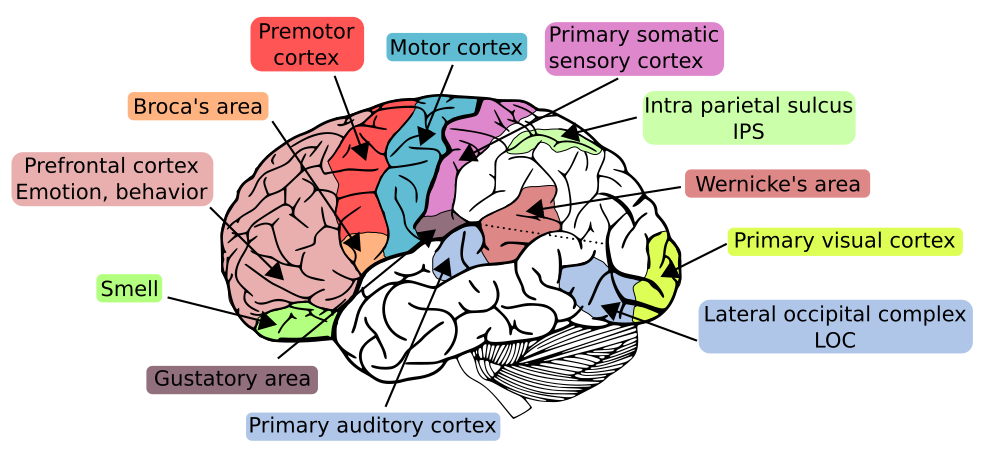
\includegraphics[width=.74\linewidth]{figures/brain_function.png}    
    \caption{\textbf{Views of the brain} at different levels of detail. The brain is composed of (spatially connected) regions and  such regions are in turn composed of populations of neurons.
      %
\textbf{Left:} Simplified view of a neuron.
A neuron (there are many types) has a cell body
called the \textit{soma}, many regions for receiving information from other neural cells
called \textit{dendrites}, and often an \textit{axon} (nerve
fiber) for transmitting information to other
cells (an axon can be longer than 1 meter in humans).
The information in the axon is transmitted through an electrical
signal called action potential, which is based on the electrical
properties of the neuronal membrane. Adapted from
\url{http://commons.wikimedia.org/}.
%      
\textbf{Right:} Each region is associated with a particular function
such as sensory areas (e.g.  visual cortex, auditory cortex) that
receive and process information from sensory organs, motors areas
(e.g. primary motor cortex, premotor cortex) that control the
movements of the subject, and associative areas (e.g. Broca’s area,
Wernicke's area) that process the high-level information related to
language production and understanding or the Intra Parietal Sulcus
--IPS-- that processes spatial information.
Adapted from \url{http://agaudi.files.wordpress.com/}.
}
\label{fig:neuron}
\end{pagefigure}

\begin{itemize}
  \item \textit{Which parts of the brain are in-charge of processing mathematical formulae as opposed to ordinary natural language ?}
  \item \textit{Which parts of the brain increase/decrease their activity when the brain is at rest ?}
  \item \textit{What are the neuro-biological markers of neurological or psychiatric mental illness ?}
  \item \textit{How does the brain structure (sulci, gyri, etc.) and function change during aging ? etc.}
 \item \textit{How do the language-responsive regions of one subject compare with that of another ? Can they be registered anatomically ?}
 \item \textit{How are the different motor or cognitive functions (language, emotion, etc.) distributed over the brain, in terms of regions and networks of regions ?}
 \item \textit{How are numbers represented and manipulated in the brain ?}
\item \textit{How does the brain and behavior change under the attack of a disease (e.g schizophrenia or a neuro-degenerative disease)}   
\end{itemize}
Note that this list is by no way exhaustive.

In the last three decades, mapping brain functional connectivity from
functional Magnetic Resonance Imaging (MRI) data has become a very
active field of research. However, analysis tools are limited and many
important tasks, such as the empirical definition of brain networks,
remain difficult due to the lack of a good framework for the
statistical modeling of the data used to define these networks.
%
% We propose to develop population models of anatomical and functional connectivity
% data to improve the alignment of subjects brain structures of interest while inferring an average template
% of these structures.
% Based on this essential contribution, we will design new statistical inference procedures to
% compare the functional connections between conditions or populations and improve the sensitivity of connectivity
% analysis performed on noisy data.

\paragraph{Objectives.} The goal of this PhD thesis is to develop new statistical methods for studying inter-subject variability (eg. amplitude of activation, size of activation clusters, topography of activation maps, etc.), the prime goal being to improve the analysis of functional connectivity in the human brain at the population level. It turns out that these concerns naturally lead to problems related to data-driven extraction of functional atlases, multivariate models for brain decoding and segmentation, and inter-subject registration of functional MRI images.

% Finally,
% we test and validate the methods on multiple datasets and
% distribute them to the brain imaging community.

% In many scientific fields, the data acquisition devices have benefited from hardware improvement to increase the resolution of the observed phenomena, leading to ever larger datasets (both in sample size $n$ and dimensionality $p$). These are the so-called ``big-data'' regimes in which
% $min(n, p) \rightarrow \infty$  and $n \ll p$ simultaneously.
% %% While the dimensionality has increased,
% %% the number of samples $n$ available is often limited, due to physical or financial limits.
% Things become instantly problematic both computationally and statistically when these
% data are processed with estimators that have a large complexity in the data size, such as
% mass-univariate models.
% In such cases, it is very useful to rely on structured priors, so that the results reflect the state of knowledge on the phenomena of interest, and we avoid sampling from empty regions of the likelihood landscape. The study of human brain activity through high-field MRI belongs to
% this class of problems.
% However, we are missing fast estimators for multivariate models for brain decoding or the study of inter-subject variability,  with structured priors, that furthermore provide statistical control on the solution.


\section{Sketch of contributions}
\label{sec:contrib}
During the preparation of this PhD project, I have authored and co-authored a number of papers in conferences and journals (including NIPS, ICASSP, MICCAI,
Frontiers in Neuroscience, etc.).
A complete least of my publications can be found on my Google scholar page \url{https://scholar.google.fr/citations?user=FDWgJY8AAAAJ&hl=fr}. In figures,
\begin{shaded}
\begin{itemize}
\item Total citations $\ge 194$.
  \item Total papers (including co-authored papers) $\ge 15$.
  \item h index $\ge 4$.
  \item 110 index $ \ge 3$.
  \end{itemize}
\end{shaded}  
Below, I  have roughly classified my main contributions under their respective sub-fields of relevance. Viz,
\begin{shaded}
\begin{itemize}
  \item{Sparsity and spatial regularization:}
     ~\citep{dohmatob2014benchmarking},  \citep{dohmatob2015speeding},
     ~\citep{abrahamregion},  ~\citep{eickenberg2015total},
     ~\citep{pelle2016multivariate}
  \item{Registration of brain images:}
    ~\citep{dohmatob2016epi2epi}
  \item{Optimization:}
     ~\citep{dohmatob2015local},  ~\citep{varoquaux2015faasta},  ~\citep{dohmatob2015simple}
  \item Modeling inter-subject functional variability:
     ~\citep{dohmatob2016}
  \item{Neuroscience:}
     ~\citep{rahim2015integrating},  ~\citep{thirion2014fmri}
  %\item{Others:}  ~\citep{Intheory,Youcrackunderpressure!}
\end{itemize}
\end{shaded}

There are also a number of preprints currently being prepared for journal publication:

\begin{shaded}
\begin{itemize}
  \item{Sparsity and spatial regularization:}
     \textit{``Structured penalties for brain decomposition and decoding: a unified view''}
   \item \textit{``Inter-subject registration of functional images: do we need anatomical images ?''}
   \item \textit{``Enhanced prediction of task-based activation maps
     from resting-state data''}
\end{itemize}
\end{shaded}


\section{Organization of the manuscript}
In this report, I shall present a selection~\footnote{For example, I shall not talk on excursional work I did on algorithmic non-cooperative game theory~\citep{dohmatob2015simple}.} of the work I have done during the preparation of my PhD project.  This selection will be centered around
\begin{itemize}
\item \textbf{Part I:} General preliminaries on neurosciences and neuro-imaging methodology $\implies$ chapter \ref{chap:bigpic}.
\item \textbf{Part II:} Structured penalties for brain decoding $\implies$ chapters \ref{chap:structured_priors}, \ref{chap:efficient_opt}, \ref{chap:speeding}, \ref{chap:igraphnet}, \ref{chap:admm}.
\item \textbf{Part III:} Functional inter-subject variability $\implies$ chapters \ref{chap:func_var}, \ref{chap:proxdict}, \ref{chap:epi2epi}, \ref{chap:rsfmri2tfmri}
\item \textbf{Conclusion:} Summary and concluding remarks $\implies$ chapter \ref{chap:conclusion}.
\end{itemize}
My precise contributions in these domains will be comprehensively outlined  as we proceed.
% I will conclude the manuscript with a synthesis of the progress made so far, and detailed plans for
% the future.

\bibliographystyle{plainnat}
\bibliography{bib_all}
